\headline{{\textbf{\Large\sffamily Tree of the Month (TOTM)}}\\
          {\textbf{\large\sffamily Monthly Themes \& Club Activities}}}
\phantomsection
\label{2026-01-themes}
\noindent
Unless stated otherwise, all events will be held in the Trimble Lounge at Whitton Community Centre on Percy Road, TW2 6JL.

%\topic{December 2025}
%\begin{itemize}
%    \item \textbf{Club Meeting:} \textit{Thursday 11th December 2026, 7pm.}
%    \item \textbf{Monthly Theme:} \textit{Festive fun \& Party time!}
%    \item \textbf{Member Education Programme:} \textit{Saturday 13th December 2025, 10am: winter structural pruning \& wiring.}
%\end{itemize}

%\topic{January 2026}
%\begin{itemize}
%    \item \textbf{Club Meeting:} \textit{Thursday 8th January 2026, 7pm.}
%    \item \textbf{Monthly Theme:} \textit{Naked tree, Elm.}
%    \item \textbf{Club Activities:} \textit{Wire application.}
%    \item \textbf{Member Education Programme:} \textit{Saturday 17th January 2026, 10 am: repotting.}
%\end{itemize}

\topic{February 2026}
\begin{itemize}
    \item \textbf{Club Meeting:} \textit{Thursday 12th February 2026, 7pm.}
    \item \textbf{Monthly Theme:} \textit{Formal / Informal styles.}
    \item \textbf{Club Activities:} \textit{Repotting, wiring, and grafting.}
\end{itemize}

\topic{March 2026}
\begin{itemize}
    \item \textbf{Club Meeting:} \textit{Thursday 12th March 2026, 7pm.}
    \item \textbf{Monthly Theme:} \textit{Carved material, jin or uro features.}
    \item \textbf{Club Activities:} \textit{Afternoon workshop with John Hanby; evening talk.}
\end{itemize}

\topic{April 2026}
\begin{itemize}
    \item \textbf{Club Meeting:} \textit{Thursday 9th April 2026, 7pm.}
    \item \textbf{Monthly Theme:} \textit{Flowering species.}
    \item \textbf{Club Activities:} \textit{Styling and repotting.}
\end{itemize}

\topic{May 2026}
\begin{itemize}
    \item \textbf{Club Meeting:} \textit{Thursday 14th May 2026, 7pm.}
    \item \textbf{Monthly Theme:} \textit{Shohin and Mame.}
    \item \textbf{Club Activities:} \textit{Talk on watering and feeding.}
\end{itemize}

\topic{June 2026}
\begin{itemize}
    \item \textbf{Club Meeting:} \textit{Thursday 11th June 2026, 7pm.}
    \item \textbf{Monthly Theme:} \textit{Deciduous species.}
    \item \textbf{Club Activities:} \textit{Three\--point display (proposed).}
\end{itemize}

\topic{July 2026}
\begin{itemize}
    \item \textbf{Club Meeting:} \textit{Thursday 9th July 2026, 7pm.}
    \item \textbf{Monthly Theme:} \textit{Larch.}
    \item \textbf{Club Activities:} \textit{Personal tree work.}
\end{itemize}

\topic{August 2026}
\begin{itemize}
    \item \textbf{Club Meeting:} \textit{Thursday 13th August 2026, 7pm.}
    \item \textbf{Monthly Theme:} \textit{Multi\--trunk trees.}
    \item \textbf{Club Activities:} \textit{Summer pruning and treatments.}
\end{itemize}

\topic{September 2026}
\begin{itemize}
    \item \textbf{Club Meeting:} \textit{Thursday 10th September 2026, 7pm.}
    \item \textbf{Monthly Theme:} \textit{Pines.}
    \item \textbf{Club Activities:} \textit{Afternoon workshop with Caz; evening talk.}
\end{itemize}

\topic{October 2026}
\begin{itemize}
    \item \textbf{Club Meeting:} \textit{Thursday 8th October 2026, 7pm.}
    \item \textbf{Monthly Theme:} \textit{Windswept or root\--over\--rock styles.}
    \item \textbf{Club Activities:} \textit{Personal tree work.}
\end{itemize}

\topic{November 2026}
\begin{itemize}
    \item \textbf{Club Meeting:} \textit{Thursday 12th November 2026, 7pm.}
    \item \textbf{Monthly Theme:} \textit{Cascade / semi\--cascade or autumn colour.}
    \item \textbf{Club Activities:} \textit{Evening with Peter Warren.}
    \item \textbf{Annual General Meeting}: \textit{Thursday 26th November 2026.}
\end{itemize}

\topic{December 2026}
\begin{itemize}
    \item \textbf{Club Meeting:} \textit{Thursday 10th December 2026, 7pm.}
    \item \textbf{Monthly Theme:} \textit{Festive fun \& party time!}
    \item \textbf{Club Activities:} \textit{Eating pizza \& drinking wine.}
\end{itemize}

\noindent \textbf{Notice:} The\textbf{Tree of the Year for 2026} is \textbf{\textit{Acer}}. 
All Acer trees entered into the Tree of the Month competition during the year will be considered for the Tree of the Year honourable mention. 
The Acer entry achieving the highest cumulative score across the competition year will be recognised as the Tree of the Year.

\closearticle

%\vfill
\headline{{\textbf{\Large\sffamily Wood You Believe It?}}\\
          {\textbf{\large\sffamily Cultivating Your Bonsai IQ}}}
\begin{itemize}
    \item \textbf{Jin and Shari:} These techniques involve creating \textbf{deadwood} on a tree.
    A ``Jin'' is a bare, stripped branch, while a ``Shari'' is a strip of deadwood on the trunk.
    Both simulate the weathering effects of harsh mountain environments.

%    \item \textbf{The Apex:} This is the highest point of the tree.
%    A well\--designed apex should be slightly rounded or ``domed'' rather than a sharp point, suggesting the maturity of a tree that has ceased its upward growth spurt.

%    \item \textbf{Yamadori:} This term refers to trees \textbf{collected from the wild}.
%    Often stunted by wind, animals, or poor soil, these specimens possess natural character and weathered features that take decades to replicate in a nursery.

%    \item \textbf{Mame and Shohin:} These are classifications of size.
%    \textbf{Shohin} trees are generally under 25cm tall, while \textbf{Mame} (meaning ``bean'') refers to palm\--sized miniatures, often under 10cm, requiring precise care.

    \item \textbf{Wound Healing:} Unlike animals, trees don't ``repair'' tissue; they \textbf{compartmentalize} it.
    By using ``cut paste'' on a fresh pruning wound, you encourage the tree to roll callous tissue over the scar more smoothly, maintaining a clean trunk line.

%    \item \textbf{Directional Pruning:} By selecting a bud that faces away from the trunk and pruning just above it, you can control the \textbf{direction of future growth}.
%    This allows you to ``steer'' the branch into open spaces without always relying on copper or aluminum wire.
\end{itemize}
\closearticle
%\clearpage

% \vfill
% \begin{center}
% 	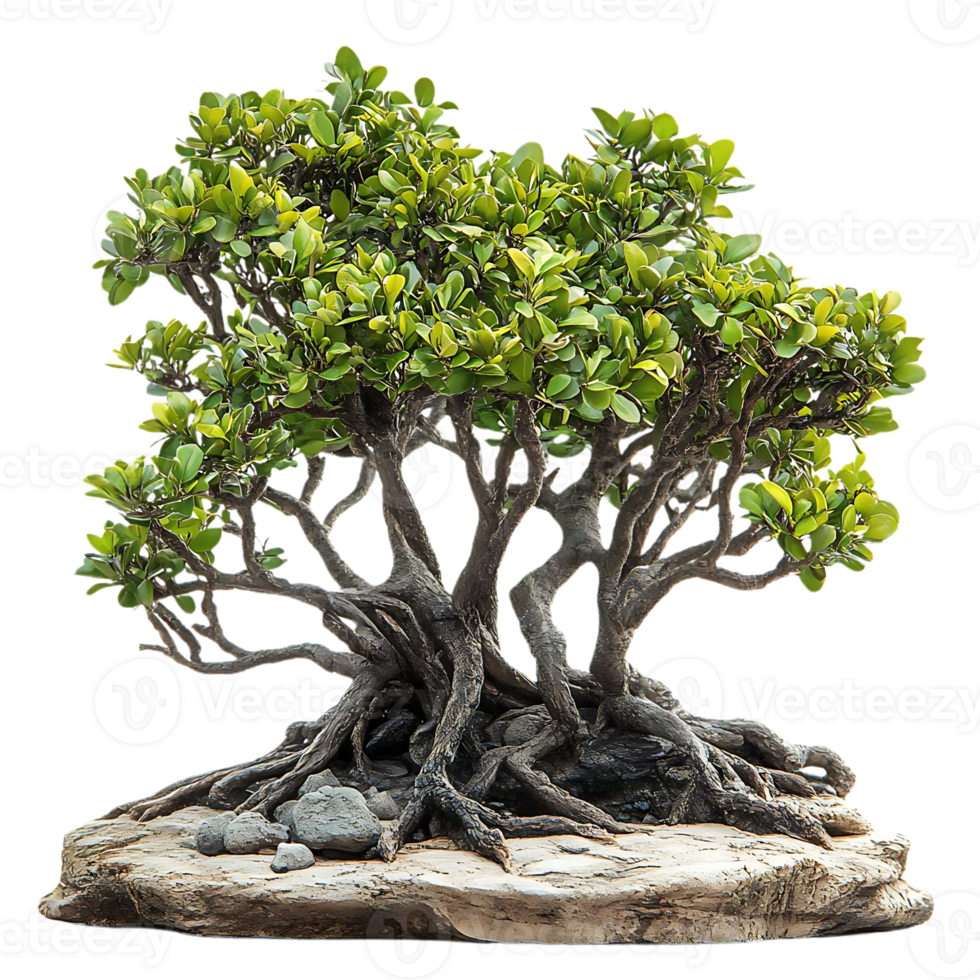
\includegraphics[width=0.95\columnwidth]{res/filler_b.png}
% \end{center}

\columnbreak
